\documentclass[11pt, letterpaper, oneside]{article}
\usepackage[utf8]{inputenc}
\usepackage{amsmath}
\usepackage{amsthm}
\usepackage{amsfonts}
\usepackage{amssymb}
\usepackage{fullpage}
\usepackage{listings}
\usepackage{xcolor}
\usepackage{graphicx}

\title{Notes on Real Time Collision Detection}
\author{Mauricio Andres Rovira Galvez}
\date{\today}

\lstdefinestyle{codestyle}{
  belowcaptionskip = 1\baselineskip,
  breaklines = true,
  frame = L,
  xleftmargin = \parindent,
  language = C++,
  showstringspaces = false,
  basicstyle = \footnotesize\ttfamily,
  keywordstyle = \color{blue}\ttfamily,
  stringstyle = \color{red}\ttfamily,
  commentstyle = \color{green}\ttfamily
}

\begin{document}
  \maketitle

  \section{Introduction}
    The topic of collision detection is of particular importance in several
    branches within computer graphics. Some examples include:
    \begin{itemize}
      \item It is used in video games to create realistic animations and 
        interactions.
      \item It is used to render a frame in a movie.
      \item It is used in general animations.
      \item It is used in physical simulations.
    \end{itemize}

    As a result, a lot of study has been devoted to this area. In these notes we
    will discuss two main components: collision detection and space partitioning
    algorithms.

    Before we begin, it is important to determine what we would want in a
    collision detection system, as well as which are the challenges that we will
    face when designing it.

      \subsection{Design Factors}
        The first thing to consider is how objects are being represented. For
        the most part, they are represented as triangular meshes (since this is
        what graphics hardware is designed to work on). That being said, there
        are other ways of representing objects, such as modelling with implicit
        functions. While the choice of representation does affect the way the
        collisions (and other algorithms) will work, let us agree to only
        consider triangular meshes for the remainder of this discussion.

        The second point of discussion is what we are going to be colliding. To
        be more concise, do we use the rendering mesh or something else?
        Let's look at an example: suppose that we have a mesh that is composed
        by 2,000,000 triangles. We wish to intersect this mesh against another
        model that is also composed of 2,000,000 triangles. The n\"aive way of
        performing this task would be to check every triangle in the first mesh
        against every triangle in the second. This, however, results in
        4,000,000,000,000 intersection tests! Even with the most powerful
        computers available, this would take a while. Even worse, it this were
        part of a game, the amount of time the player would have to wait
        \emph{per} frame is unacceptable. 

        Clearly in this case we would want to use something \emph{other} than
        the render mesh, preferably something that is more compact. This is
        where bounding volumes kick in. These volumes are called proxy geometry.
        These are usually optimized for collision detection systems.
        Unfortunately, they also represent a problem: suppose that all of the
        proxies are computed in a pre-processing step. What happens when the
        original mesh is altered? How do we maintain these new geometries?

    \section{Bounding Volumes}
      In this section we will discuss bounding volumes. In particular, we will
      be focusing on the following three:
      \begin{enumerate}
        \item Axis-aligned bounding boxes (AABB),
        \item spheres,
        \item and oriented bounding boxes (OBB).
      \end{enumerate}

      We begin our discussion of bounding volumes by asking the following
      question: what kind of properties do we want in a bounding volume?
      Ideally, we would want the following:
      \begin{itemize}
        \item Inexpensive intersection tests.
        \item Tight fitting.
        \item Inexpensive to compute.
        \item Easy to transform (rotations are of particular importance).
        \item Use little memory.
      \end{itemize}

      Unfortunately as we will soon see, there have to be trade-offs whenever we
      select a bounding volume. For example: a sphere is trivial to test and
      occupies little memory (it only requires 4 floats). Conversely, a convex
      hull gives us a very tight bound on the object, but requires a lot more
      memory and is more expensive to test for intersections. So the choice of
      bounding volume ultimately boils down to the specific requirements of our
      application.

      \subsection{Asis-aligned Bounding Boxes}
        This is one of the most common bounding volumes used today. It is
        characterized by having each one of its faces aligned with the given
        coordinate systems. In other words, the face normals will always be
        parallel with the axes of the coordinate system.

        There are three common ways to represent an AABB as shown below:
        \begin{figure}[h]
          \caption{The three common AABB representations: (from left to right)
          min-max, min-widths, and centre-radius.}
          \label{aabb_representations}
          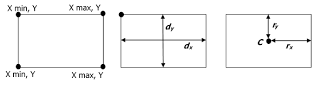
\includegraphics[width=\textwidth]{images/aabb_representations}
        \end{figure}

        In terms of storage, the centre-radius representation is the most
        efficient, since we can store the array of halfwidths with less bits
        than the centre position values. The worst is the min-max
        representation, since it requires all 6 values to be stored (usually as
        floats, but they could be doubles). In terms of updating the volume, the
        last two are the easiest to maintain, while the min-max requires us to
        translate both points, as opposed to just one.

        The intersection test for AABBs is very straight-forward and most of the
        optimizations here boil down to either re-ordering of the if-statements,
        or optimizing (if it isn't already) the absolute value function.

      \subsection{Computing and Updating AABBs}
        We generally define AABBs in terms of the model space for the particular
        object. This poses an interesting problem: when we want to perform an
        intersection test between two different objects, we must transform both
        AABBs to a common space. The question is: which one?
        
        The reason why this question is interesting is because it is completely
        possible to construct a case where objects intersect (or not) depending
        on the choice of space. On top of this, whenever we transform an object
        from one space to another we are essentially translating them. This
        translation introduces error into the calculations, which at times may
        be avoided entirely by selecting a space that leaves the objects close
        (or on) the origin.

        Some bounding volumes (such as convex hulls) are free from orientation,
        while AABBs are not. This means that whenever an object is rotated, the
        AABB must be updated in order to preserve its alignment to the axes.
        The most common strategies for this are:
        \begin{itemize}
          \item Use a loose-fitting AABB that always encloses the object.
          \item Compute a tight dynamic reconstruction from the original set.
          \item Computing a tight dynamic reconstruction using hill climbing.
          \item Computing an approximate dynamic reconstruction from the
            rotated AABB.
        \end{itemize}
        Let us examine each one in a bit more detail.

        The first option is to essentially construct an AABB that contains the
        bounding sphere for that particular mesh. This means that any rotation
        can be ignored, since spheres are invariant under rotation. This
        approach has the big drawback of not being particularly tight, and it
        would be easier (in some cases) to just use the bounding sphere directly
        instead of wrapping it in an AABB.

        Reconstructing an AABB from the point set involves iterating over all
        the vertices and finding the one that has the smallest and largest
        points along each of the axes. As you might expect, this is an $O(n)$
        operation. It is possible to optimize this by removing all the points
        that do not lie on the convex hull of the object (since the bounding box
        must contain points that lie on the convex hull). This requires some
        pre-processing that needs to be done on the object prior to constructing
        the AABB. This may not be worth the time (or the memory) it takes to
        perform these operations, so it may be worth investigating a better
        bounding volume.

        Another way of optimizing the reconstruction of an AABB requires a way
        to easily obtain the neighbourhood of a specific vertex. Given this, we
        can construct an AABB by maintaining 6 pointers to the most extreme
        points in each of the axes. Whenever we rotate the object, we climb
        along the neighbours of the old vertex until we find a new extremal
        point. This has an obvious drawback: the objects must be convex in order
        for this to work properly (otherwise we would get stuck in local minima
        and would never find the new extremal point). We can further optimize
        this by reducing the number of comparisons we have to perform. For
        example, if we are looking for the maximal point in $+x$, then we only
        need to look at the $x$ coordinate of the vectors. The other obvious
        problem is that hill-climbing requires a robust implementation for
        finding neighbours for any given vertices.

        The last of the four realignment methods is to simply wrap the rotated
        AABB in a new AABB. This gives us a new (approximate) AABB that we can
        use to compute our collision detections. It is important to keep in mind
        that the new AABB \emph{must} be computed with respect to the original
        AABB, otherwise the box will just grow indefinitely.
        The idea is as follows: consider a box $A$ that was transformed by a
        matrix $\mathbf{M}$ resulting in a box $A'$. The three columns (or rows
        depending on the convention) contain the world-coordinate axes of $A'$
        in its local frame. \\
        So what does this all mean? Well suppose that $A$ is given using min-max
        representation and $\mathbf{M}$ is a column matrix. This means that we
        can find the extents of $B$ by simply projecting each of the rotated
        vertices onto the world-coordinate axes. Since minimal and maximal
        extents will be composed by a linear combination of the transformed
        values of $A$, then it is only a matter of finding the new min and max.
        This can be easily done by adding the smaller terms and the largest
        terms (respectively).

      \subsection{Spheres}
        Spheres are another very common bounding volume. Like AABBs, the
        intersection tests for spheres is very simple to perform. In addition,
        spheres have the property that they are invariant under rotations, which
        means that the only transformation that affects them is translation,
        which is very simple to do. They also have a very compact
        representation: we only need a point and a radius to fully determine a
        sphere. That said, the interesting part of spheres isn't in their
        intersection tests, but rather on how they are computed.

\end{document}
